\chapter{Perancangan}
\label{chap:perancangan}
Bab ini akan menjelaskan perancangan aplikasi visualisasi data histori KIRI pada google map

\section{Perancangan Antarmuka}
\label{sec:perancanganAntarmuka}
Pada aplikasi, disediakan antarmuka untuk memudahkan pengguna dalam berinteraksi dengan perangkat lunak \ref{fig:antarmuka}.

\begin{figure}[H]
	\centering  
	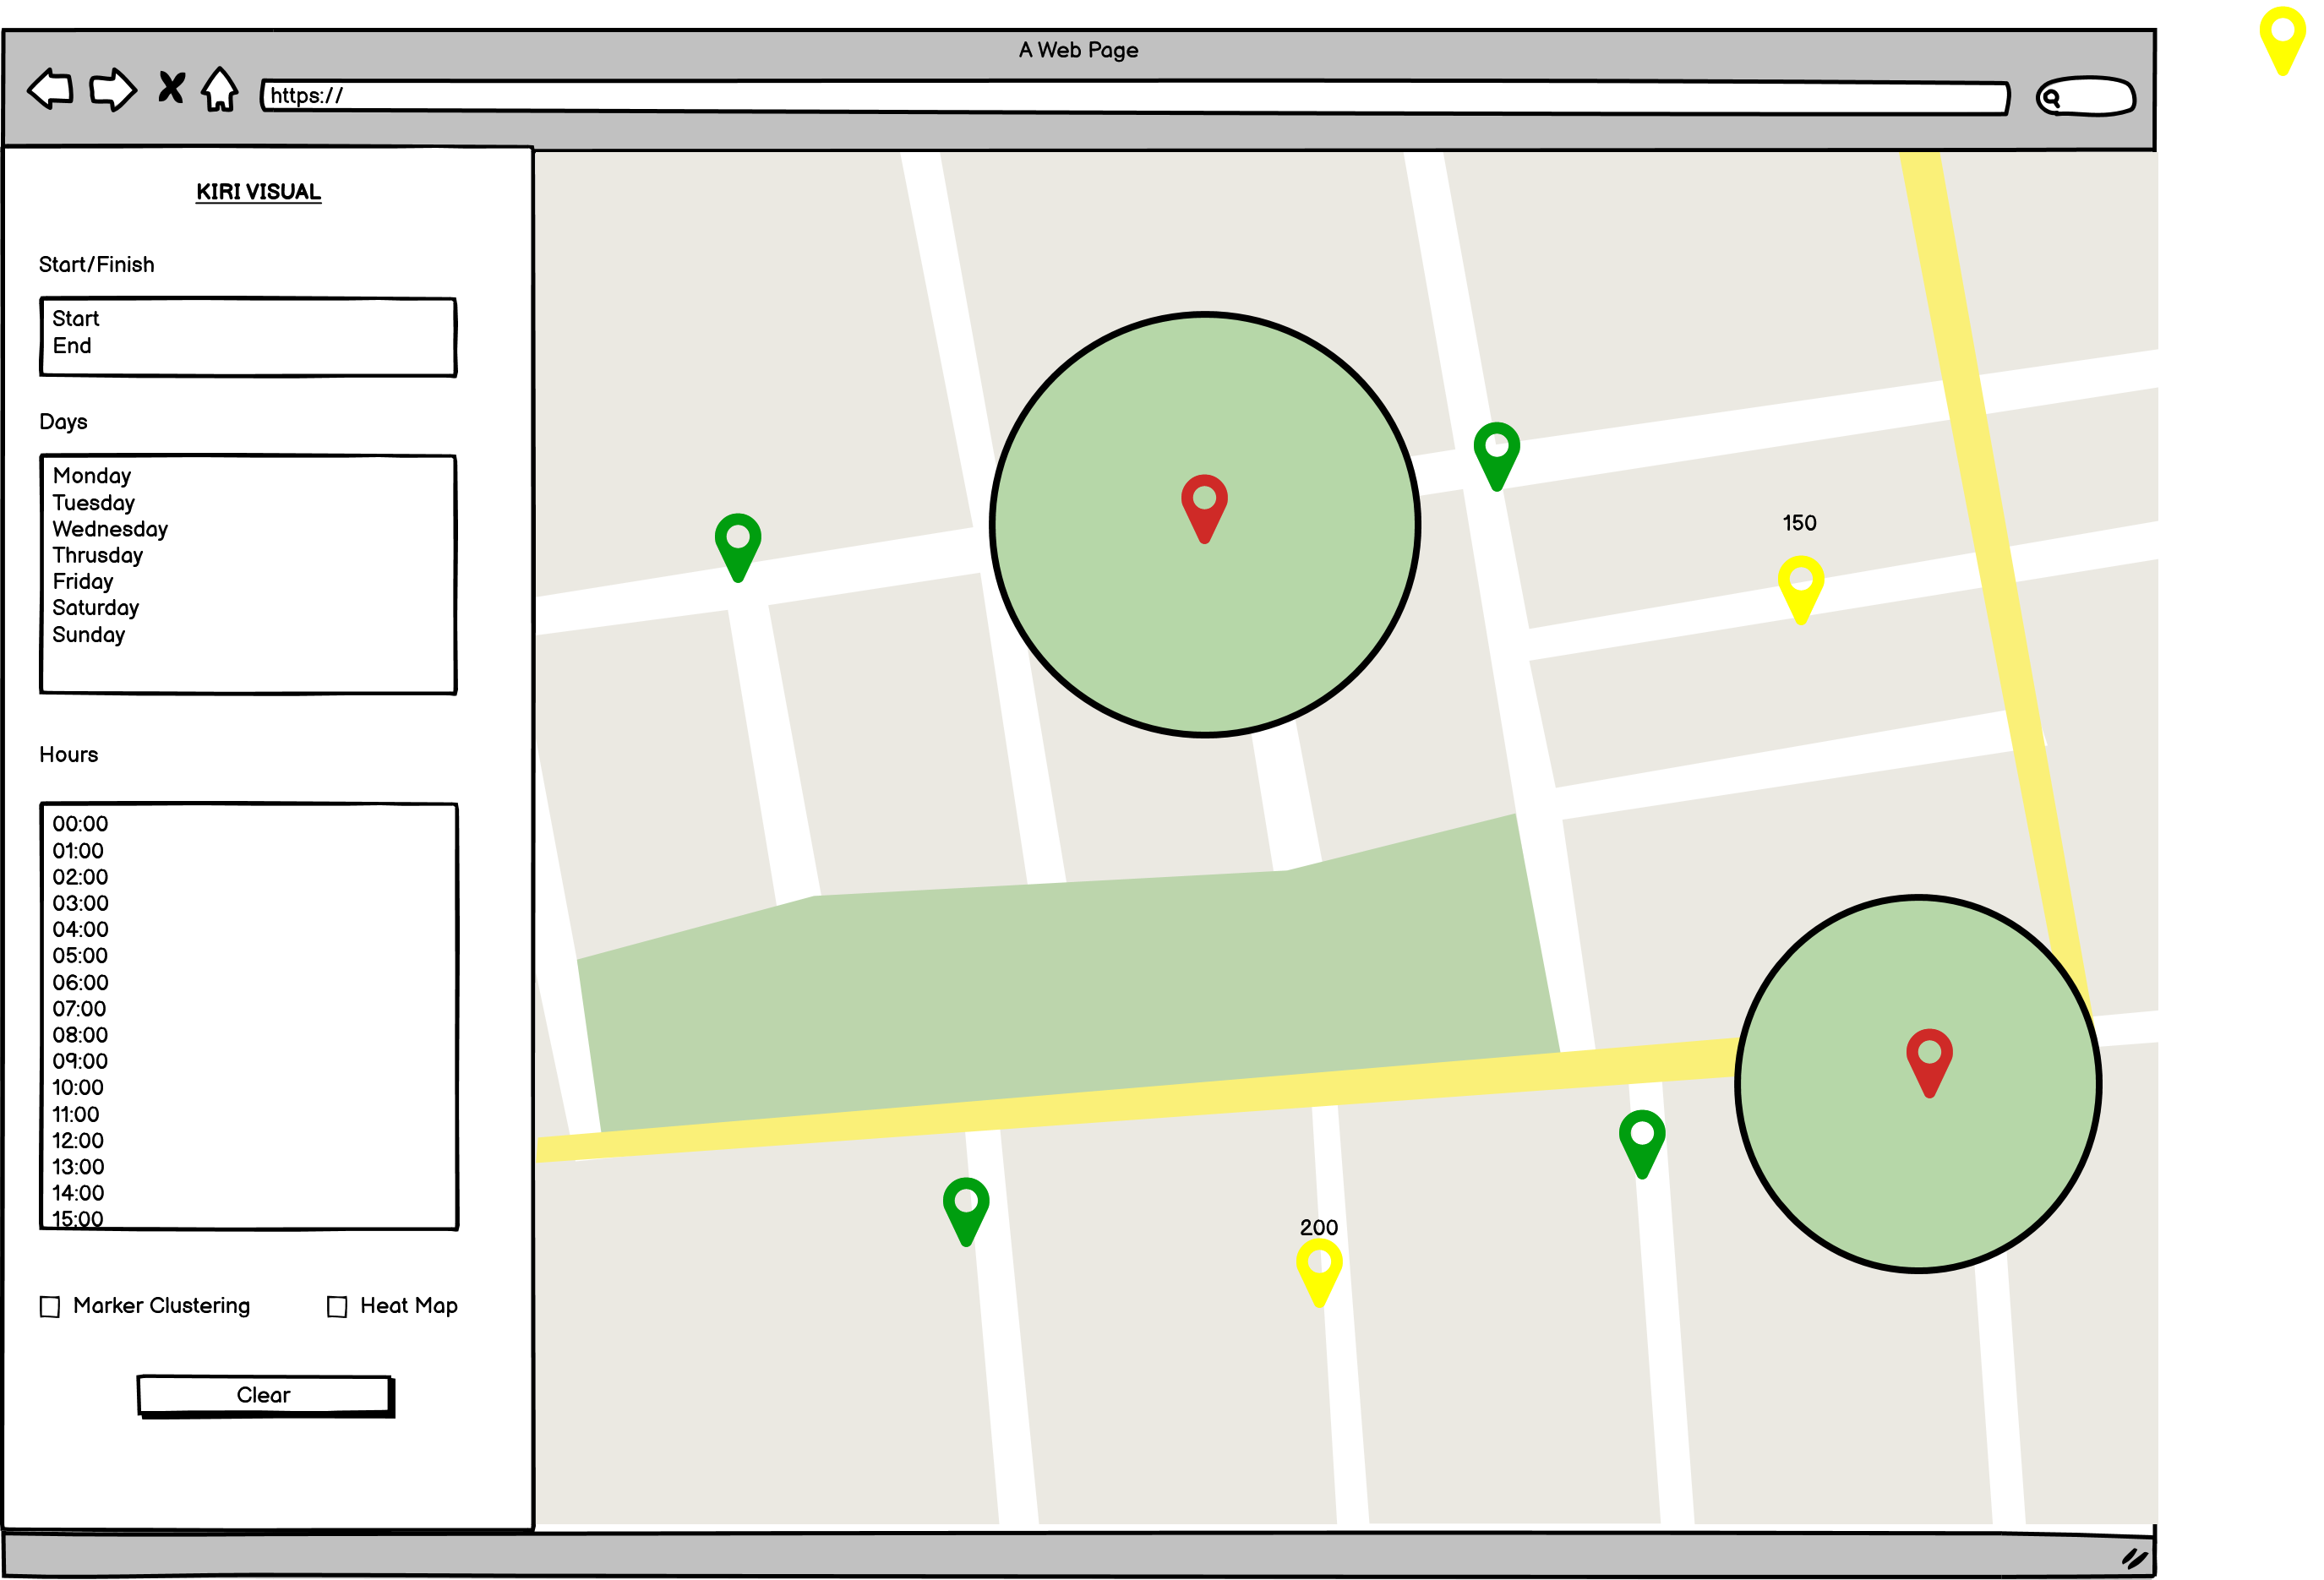
\includegraphics[scale=0.3]{Gambar/mockup.PNG}  
	\caption[Rancangan Antarmuka]{Rancangan Antarmuka} 
	\label{fig:antarmuka} 
\end{figure}

Berdasarkan rancangan diatas, berikut adalah fungsi dari setiap komponen dalam antarmuka:
\begin{itemize}
	\item \textit{Map}: digunakan untuk menampilkan peta \textit{google map}.
	\item \textit{Checkbox Start}: untuk memfilter data berdasarkan tempat keberangkatan.
	\item \textit{Checkbox End}: untuk memilfter data berdasarkan tempat tujuan.
	\item \textit{Selection Box Hours}: untuk memfilter data berdasarkan jam.
	\item \textit{Selection Box Days}: untuk memfilter data berdasarkan hari.
	\item \textit{Checkbox Heat Map}: untuk menampilkan data dalam bentuk \textit{heat map}.
	\item \textit{Checkbox Marker Clustering} : untuk menampilkan data dalam bentuk \textit{marker clustering}.
	\item Button \textit{Clear}: menghapus seluruh \textit{overlay} pada objek \textit{map}.
\end{itemize}

\section{Perancangan Diagram Fungsi}
\label{sec:perancanganDiagramFungsi}
Berdasarakan hasil analisis pada  \ref{sec:analisisKebutuhanPerangkatLunak}, maka untuk aplikasi ini dapat dibuat diagram fungsi seperti \ref{fig:diagramFungsi} 
\begin{figure}[H]
	\centering  
	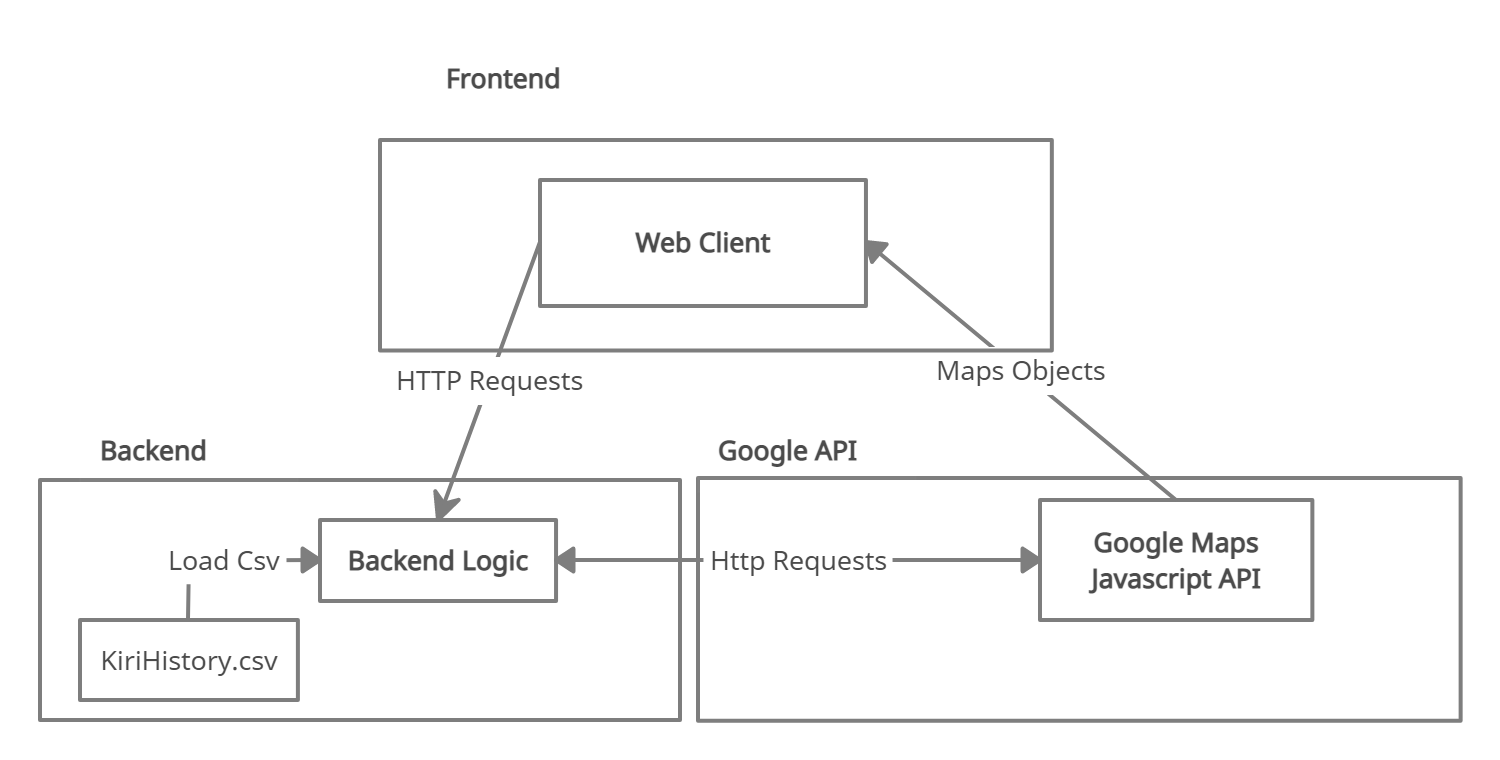
\includegraphics[scale=0.3]{Gambar/Kiri_functional_diagram.png}  
	\caption[Rancangan Diagram Kelas]{Rancangan Diagram Fungsi} 
	\label{fig:diagramFungsi} 
\end{figure}

Aplikasi ini merupakan aplikasi berbasis website dimana akan memanfaatkan \textit{node.js} yang akan berperan sebagai \textit{asynchronous event-driven} \ref{sec:nodejs} Sehingga  backend logic dapat menggunakan \textit{javascript} tanpa menggunakan \textit{web browser}. Pada aplikasi ini terdiri dari tiga bagian yakni:
\label{sec:tigakomponenet}
\begin{itemize}
    \item Frontend pada bagian frontend terdiri dari \textit{web client} yang berfungsi untuk menerima input dan mengeluarkan output dari \textit{user}. Webclient akan berkomunikasi dengan \textit{backend} dengan menggunakan \textit{http request}.
    
    \item Backend akan menggunakan \textit{node.js} akan menerima input dari web client pada bagian ini juga akan dilakukan \textit{load} data histori kiri yang berbentuk csv untuk dapat diolah.
    
    \item Google API aplikasi ini akan memanfaat \textit{google maps javascript api} untuk dapat memvisualisasikan data history KIRI.
\end{itemize}

\section{Perancangan Diagram Kapabilitas}
\label{sec:kapabilitasDiagram}
Berdasarkan kapabilitas dari masing masing komponen \ref{sec:tigakomponenet}, maka dapat dibuat diagram kapabilitas.

\subsection{Diagram Kapabilitas Web Client}
\label{sec:webclientCapability}
Pada bagian \textit{web client} akan memiliki kapabilitas:
\begin{itemize}
    \item Menampilkan Google Map.
    \item Menampilkan \textit{heatmap} atau \textit{marker clustering} object.
    \item Menerima input dari user. Input dari user berupa parameter yang berguna untuk memfilter data histori kiri dan menampilkannya dalam bentuk \textit{heatmap} atau \textit{marker clustering}.
\end{itemize}

Berdasarkan kapabilitas \ref{sec:webclientCapability} maka dapat dibuat diagram yang berbentuk seperti \ref{fig:webclientcapabiltydiagram}

\begin{figure}[H]
	\centering  
	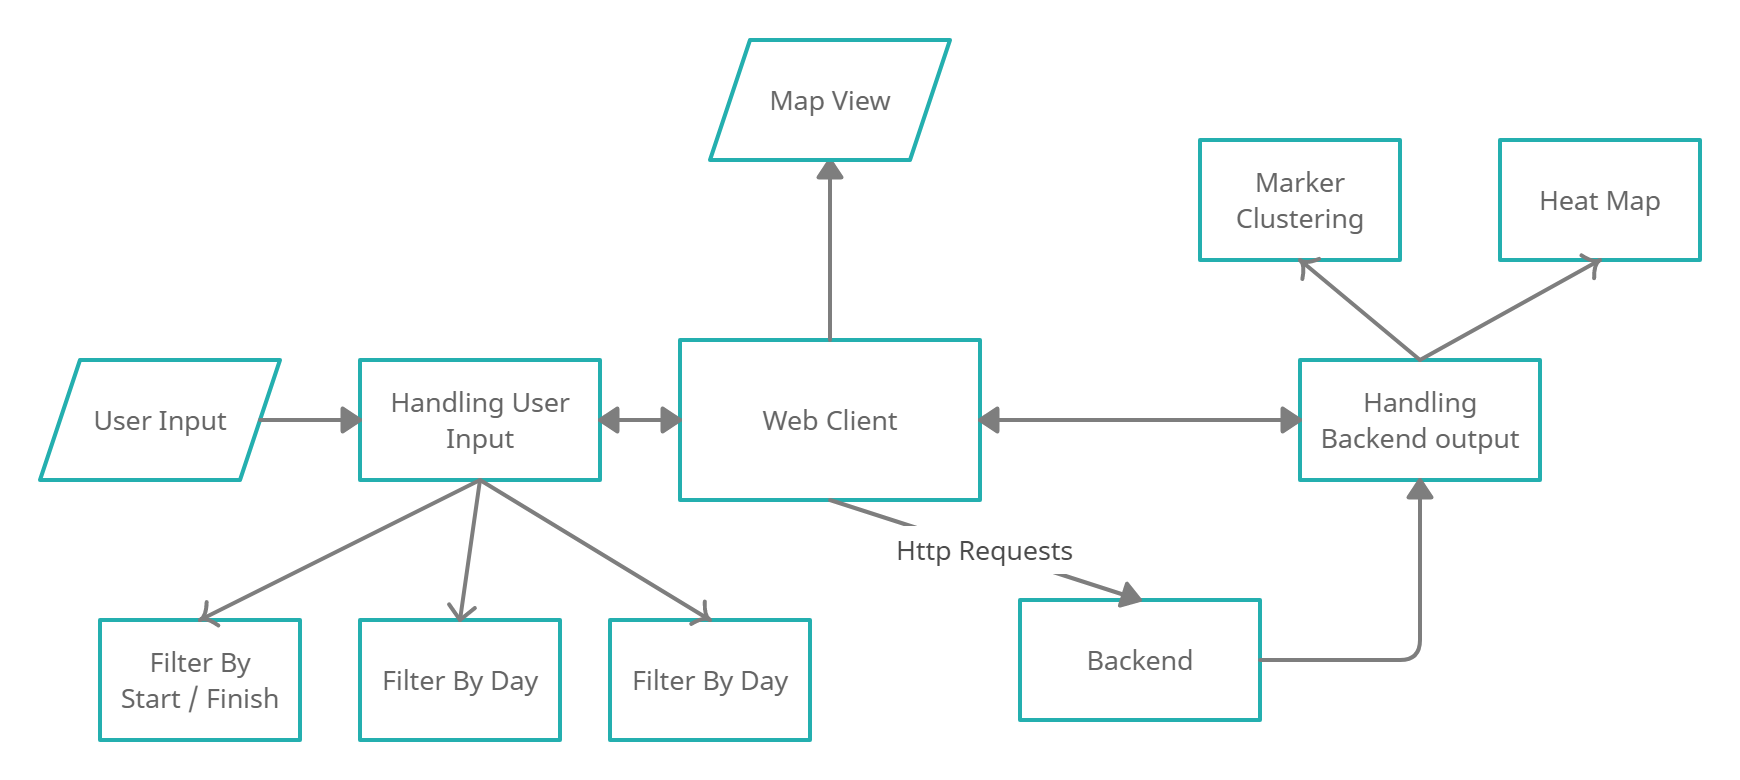
\includegraphics[scale=0.25]{Gambar/kiri_web_client_capability.png}  
	\caption[Rancangan Diagram Kapabilitas]{Diagram Kapabilitas Web Client} 
	\label{fig:webclientcapabiltydiagram} 
\end{figure}

\subsection{Diagram Kapabilitas Backend}
\label{sec:backendCapabilityDiagram}
Pada aplikasi yang akan dibangun backend memiliki kapabilitas:
\begin{itemize}
    \item Menerima \textit{input} dari \textit{web client}. Input yang diterima berupa filter parameter yang telah diolah oleh \textit{web client}.
    \item Melakukan filterisasi data berdasarkan \textit{input parameter} dari \textit{web client}.
    \item Melakukan komunikasi \textit{via http request} terhadap \textit{google api}.
\end{itemize}

Berdasarkan kapabilitas \ref{sec:backendCapabilityDiagram} maka dapat dibuat diagram yang berbentuk seperti \ref{fig:backendCapabilityDiagram}

\begin{figure}[H]
	\centering  
	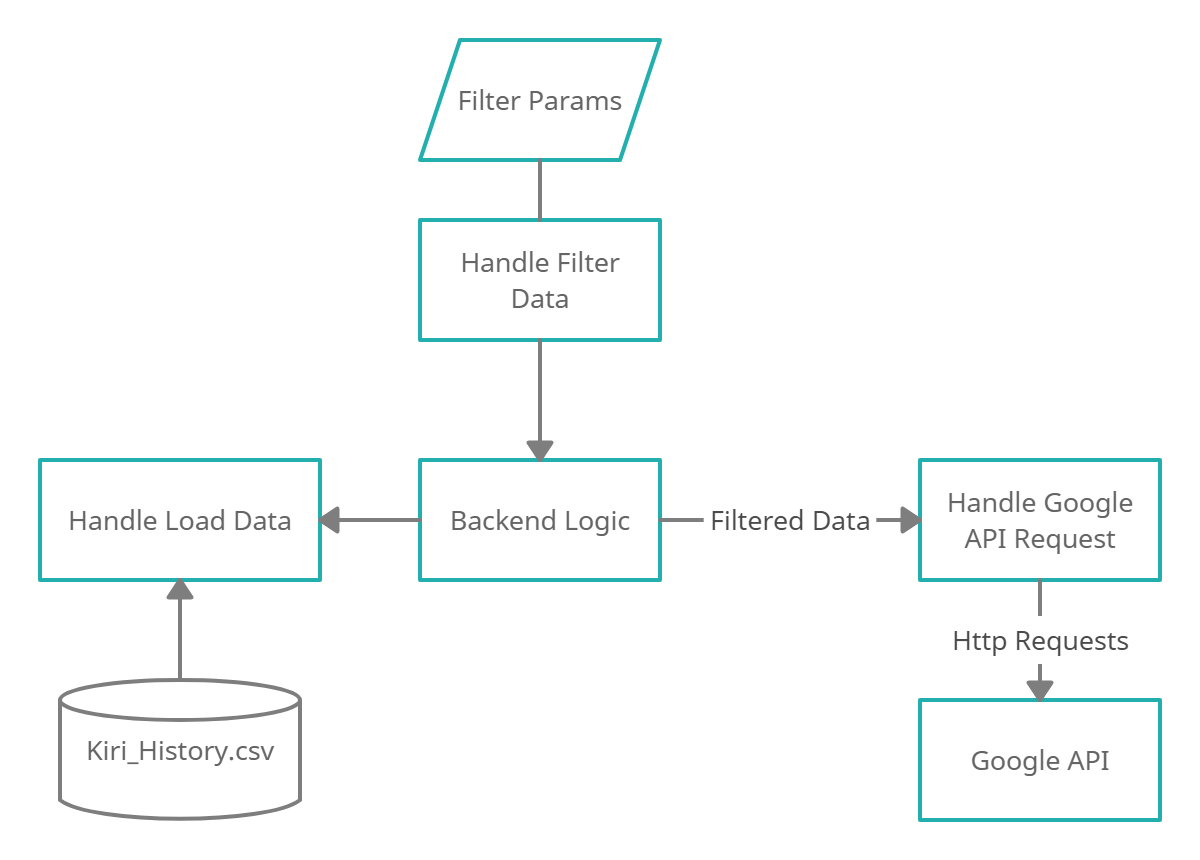
\includegraphics[scale=0.25]{Gambar/Kiri_Backend_Capabilty.png}  
	\caption[Rancangan Diagram Kapabilitas]{Diagram Kapabilitas Backend} 
	\label{fig:backendCapabilityDiagram} 
\end{figure}

\subsection{Diagram Kapabilitas Google API}
\label{sec:googleCapabilityDiagram}
Pada aplikasi ini akan menggunakan \textit{google maps javascript api} sebagai \textit{third party library} dalam menampilkan hasil visualisasi data yang dilakukan oleh \textit{backend}. \textit{Google Maps Javascript API} pada perangkat lunak ini memiliki kapabilitas antara lain:
\begin{itemize}
    \item Menerima \textit{input} dari \textit{Backend}. Input yang diterima berupa data histori kiri yang telah disaring sesuai dengan  \textit{input} dari user.
    \item Mengeluarkan \textit{output} berupa objek \textit{map} yang akan dirender oleh \textit{web client}. Objek \textit{map} dapat berupa \textit{marker cluster} objek atau \textit{heatmap} objek tergantung pada input yang diterima dari \textit{backend}.
\end{itemize}
Berdasarkan kapabilitas \ref{sec:googleCapabilityDiagram} maka dapat dibuat diagram yang berbentuk seperti \ref{fig:googleCapabilityDiagram}

\begin{figure}[H]
	\centering  
	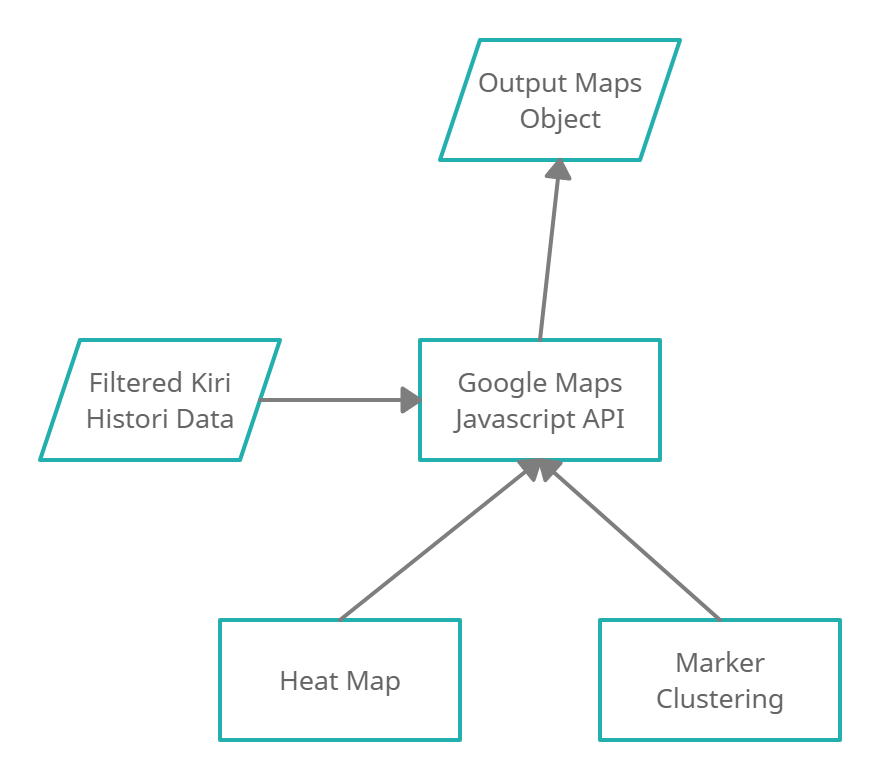
\includegraphics[scale=0.25]{Gambar/Kiri_GoogleAPI_Capabilty.png}  
	\caption[Rancangan Diagram Kapabilitas]{Diagram Kapabilitas Goolge API} 
	\label{fig:googleCapabilityDiagram} 
\end{figure}

\section{Perancangan Diagram Interaksi}
Pada subbab ini akan dijelaskan interaksi antar komponen yang  sesuai dengan yang dijelaskan pada subbab \ref{sec:deskripsiPL}, dengan diagram interkasi untuk setiap fitur pada aplikasi visualisasi data histori kiri.


\begin{figure}[H]
	\centering  
	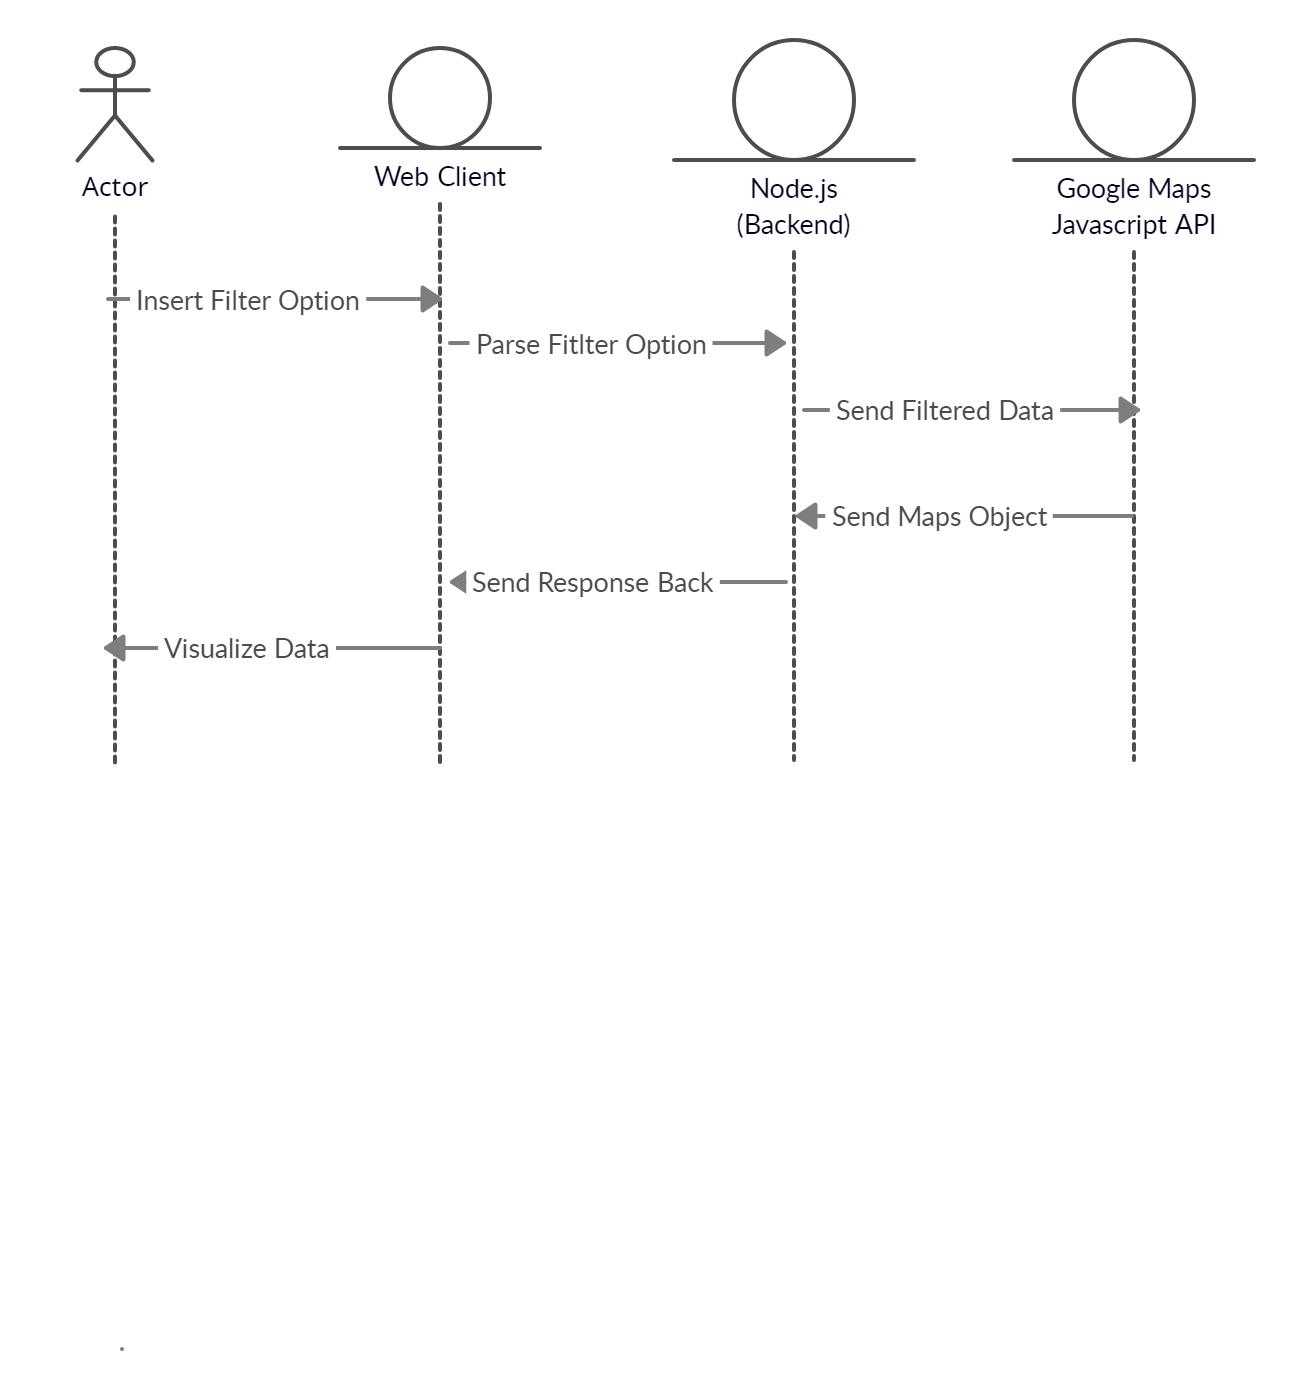
\includegraphics[scale=0.3]{Gambar/Kiri_Sequence_Diagram.png}  
	\caption[Rancangan Diagram Interaksi]{Diagram Interaksi Visualisasi Data Histori Kiri} 
	\label{fig:interactionDiagram} 
\end{figure}

Fitur pada perangkat lunak ini akan diawali dengan user dapat memilih \textit{input filter}. \textit{Input filter} yang dapat dipilih adalah filter berdasarkan atribut \textit{start} atau \textit{finish}, \textit{days}, dan \textit{time}. Setelah filter option dipilih oleh user maka \textit{web client} akan mengubah hasil option tersebut menjadi \textit{filter params}, \textit{filter params} adalah sebuah objek yang akan digunakan oleh \textit{backend logic} untuk melakukan proses \textit{filter} terhhadap data histori KIRI. Setelah \textit{backend logic} menerima \textit{filter params} maka proses \textit{filter} akan dilakukan sesuai dengan isi dari \textit{filter params}, aksi ini akan menghasilkan data histori kiri yang sudah disaring sesuai dengan isi dari \textit{filter params}. \textit{Backend logic} akan mengirimkan hasil data disaring tersebut ke \textit{google maps javascript api} dengan lalu \textit{google maps javascript api} akan mengeluarkan maps object berdasarkan data yang dikirim oleh \textit{backend logic}. Data tersebut akan ditampilkan kembali oleh \textit{web client} dalam bentuk data visualisasi menggunakan \textit{google map}.


\section{Perancangan Pseudocode}
\label{sec:psudeoCode}
Pada subbab ini dirancang \textit{pseudocode} untuk membuat aplikasi visualisasi data histori KIRI. \textit{Pseudocode} yang dibuat akan mengacu pada kapabilitas setiap komponent \ref{sec:kapabilitasDiagram}.

\subsection{Perancangan Pseudocode Pada Web Client}
\label{sec:psudeoCodeWebClient}
Berdasarkan kapabilitasnya  \ref{sec:webclientCapability}. Pseudocode dapat dibuat berdasarkan dua fungsi utama yakni:
\begin{itemize}
    \item Handling User Input. Pada tahap ini web client akan menerina input dari user dan akan mengubah nya menjadi \textit{filter params}.
    \item Menampilkan data histori kiri dengan menggunakan \textit{google maps}.
    
\end{itemize} 

\begin{table}[H]
    \centering
       \caption{Handling User Input}
    \begin{tabular}{|p{3cm}|p{10cm}|}
    \hline
        Nama & Handling User Input.\\
    \hline
    \hline
        Deskripsi & Fungsi yang bertugas untuk menerima input user dan mengubah inputan user menjadi \textit{filter params}  \\
    \hline
        Pre-kondisi & Aplikasi sudah menerima hasil input dari user.\\
    \hline
        Input & 
        Input yang akan diterima oleh aksi ini antara lain:
        \begin{itemize}
            \item \textit{Days} aksi akan menerima \textit{input days} yang bertipe \textit{array of number} dengan \textit{range} antara 0 sampai 6 yang merepresentasikan hari.
            \item \textit{Hours} aksi akan menerima \textit{input hours} yang bertipe \textit{array of number} dengan \textit{range} antara 0 sampai 23 yang merepresntasikan jam.
            \item \textit{isHeatMap} aksi akan menerima parameter bertipe \textit{boolean} yang menandakan apakah user memilih menggunakan \textit{map} bertipe \textit{heat map}.
            \item \textit{isMarkerClustering} aksi akan menerima parameter bertipe \textit{boolean} yang menandakan apakah user memilih menggunakan \textit{map} bertipe \textit{marker clustering}.
        \end{itemize}
       \\
       \hline
        Output & 
        Output yang akan dihasilkan oleh aksi ini adalah object \textit{filter params}. \textit{Filter params} merupakan sebuah objek yang memiliki dua buah atribut antara lain: 
        \begin{itemize}
            \item Atribut day atribut ini adalah atribut untuk menampung array of number yang merepresentasikan hari.
            \item Atribut hour atribut ini adalah atribut untuk menampung array of number yang merepresentasikan jam.
        \end{itemize}
       \\
    \hline
    \end{tabular}
\end{table}

\textbf{Pseudocode} untuk aksi \ref{sec:psudeoCodeWebClient} dapat digambarkan seperti:
\begin{algorithm}
\caption{Handle User Input}\label{euclid}
\begin{algorithmic}[1]
\Function{createFilterObj}{}
\State $\textit{days} \gets \text{array of }\textit{days}$
\State $\textit{hours} \gets \text{array of }\textit{hours}$
\State $\textit{filterParams} \gets \text{object of selected }\textit{input}$
\State $\textit{filterParams.days} \rightarrow \text{days}$
\State $\textit{filterParams.hours} \rightarrow \text{hours}$
\State \Return $\textit{filterParams} $
\end{algorithmic}
\end{algorithm}


\begin{table}[H]
    \centering
       \caption{Menampilkan data histori kiri dengan menggunakan \textit{google maps}}
    \begin{tabular}{|p{3cm}|p{10cm}|}
    \hline
        Nama & Handling Output.\\
    \hline
    \hline
        Deskripsi & Fungsi yang bertugas untuk menampilkan \textit{maps object} yang dikirimkan oleh \textit{backend}.
        \\
    \hline
        Pre-kondisi & Aplikasi sudah menerima objek \textit{map} dari \textit{backend}.\\
    \hline
        Input & 
        Aksi memerlukan input antara lain 
        \begin{itemize}
            \item Selected \textit{map type}. tipe \textit{map} yang dapat dipilih user adalah \textit{heat map} atau \textit{marker clustering}.
            \item Objek \textit{map} yang telah dikirimkan oleh \textit{google maps javascript api}.
        \end{itemize}
       \\
       \hline
        Output & 
        Output yang akan dihasilkan oleh aksi ini adalah hasil visualisasi dari objek \textit{map} yang diterima dari \textit{backend}. Hasil visualisasi dapat berbentuk \textit{Heat Map} atau \textit{Marker Clustering}
       \\
    \hline
    \end{tabular}
\end{table}

\begin{algorithm}[htbp]
\caption{Handle Output}
\begin{algorithmic}[1]
\Function{setMap}{isMarkerCluster,data}
\State $\textit{map} \gets \text{google maps object}$
\State $\textit{data} \gets \text{response.data}$
\If{isMarkerCluster == true}
    \State $\textit{markers} \gets \text{setMarkers(data)}$
    \State $\textit{markerCluster} \gets \text{MarkerClusterer(map , data)}$
\Else
    \State $\textit{heatMap} \gets \text{setHeatmap(data)}$
\EndIf
\EndProcedure
\end{algorithmic}
\end{algorithm}


\subsubsection{Perancangan Pseudocode Pada Backend Server}
Berdasarkan kapabilitasnya \ref{sec:backendCapabilityDiagram}.  Pseudocode dapat dibuat berdasarkan dua fungsi utama yakni:
\begin{itemize}
    \item Handling load data histori KIRI.
    \item Handling filter data histori KIRI.
\end{itemize}

\begin{table}[H]
    \centering
       \caption{Load data histori KIRI}
    \begin{tabular}{|p{3cm}|p{10cm}|}
    \hline
        Nama & Load Data.\\
    \hline
    \hline
        Deskripsi & Fungsi ini adalah fungsi yang berperan untuk meload data histori KIRI.
        \\
    \hline
        Pre-kondisi & Data histori kiri sudah tersedia didalam folder asset dan harus bertipe \textit{csv}.\\
    \hline
        Input & 
        aksi memerlukan input antara lain 
        \begin{itemize}
            \item Data histori KIRI berbentuk \textit{csv}.
        \end{itemize}
       \\
       \hline
        Output & 
        \textit{Array of Object} data histori kiri.
       \\
    \hline
    \end{tabular}
\end{table}

\begin{algorithm}[htbp]
\caption{Load Data}
\begin{algorithmic}[1]
\Function{loadData}{}
\State $\textit{data} \gets \text{array of objects}$
\State $\textit{data} \gets \text{fs.readFile("KiriHistory.csv")}$
\State \Return $\textit{data}$
\EndIf
\EndProcedure
\end{algorithmic}
\end{algorithm}


\begin{table}[H]
    \centering
       \caption{Handling Filter Data}
    \begin{tabular}{|p{3cm}|p{10cm}|}
    \hline
        Nama & Filter Data.\\
    \hline
    \hline
        Deskripsi & Fungsi ini bertugas untuk memfilter data berdasarkan filter parameter yang telah dikirimkan oleh \textit{web client}.
        \\
    \hline
        Pre-kondisi &\textit{Web client} telah mengirimkan \textit{filter param}.\\
    \hline
        Input & 
        Aksi memerlukan input antara lain 
        \begin{itemize}
            \item Filter param.
        \end{itemize}
       \\
       \hline
        Output & 
        \textit{Array of Object} data histori kiri yang telah disaring.
       \\
    \hline
    \end{tabular}
\end{table}


\begin{algorithm}[htbp]
\caption{Filter Data}
\begin{algorithmic}[1]
\Function{filterData}{filterParams}
\State $\textit{data} \gets \text{array of objects}$
\State $\textit{data} \gets \text{data.filter(filterParams)}$
\State \Return $\textit{data}$
\EndIf
\EndProcedure
\end{algorithmic}
\end{algorithm}
